\documentclass[border=10mm]{standalone}
\usepackage{tikz}
\usepackage{amsmath}
\usepackage{amssymb}
\usepackage{bm}
\usetikzlibrary{arrows.meta, fit, backgrounds, calc, positioning}

%%─── Palette ────────────────────────────────────────────────────────────────
\definecolor{tBlue}   {RGB}{52,119,196}
\definecolor{sGreen}  {RGB}{56,142,60}
\definecolor{ibOrange}{RGB}{230,130,30}
\definecolor{lossRed} {RGB}{198,40,40}
\definecolor{pPurple} {RGB}{123,31,162}
\definecolor{eGold}   {RGB}{180,140,0}
\definecolor{uwBrown} {RGB}{120,80,40}

%%─── Node styles ────────────────────────────────────────────────────────────
\tikzset{
  nd/.style  = {draw, rounded corners=4pt, align=center, inner sep=5pt,
                minimum width=3.0cm, minimum height=0.9cm, font=\small},
  T/.style   = {nd, draw=tBlue,   fill=tBlue!10},
  S/.style   = {nd, draw=sGreen,  fill=sGreen!10},
  ENC/.style = {nd, draw=eGold,   fill=eGold!15},
  IB/.style  = {nd, draw=ibOrange,fill=ibOrange!18},
  PL/.style  = {nd, draw=pPurple, fill=pPurple!12},
  PRED/.style= {nd, draw=pPurple!80, fill=pPurple!7, densely dotted,
                minimum width=2.2cm, minimum height=0.85cm},
  DR/.style  = {nd, draw=sGreen!70, fill=sGreen!4, densely dashed},
  LO/.style  = {nd, draw=lossRed, fill=lossRed!10, minimum width=2.8cm},
  LOX/.style = {nd, draw=lossRed, fill=lossRed!10, minimum width=3.0cm,
                double, double distance=1pt},
  TOT/.style = {nd, draw=uwBrown, fill=uwBrown!8, font=\small},
  Tarr/.style ={-{Stealth[length=5pt]}, thick, tBlue!60,  dashed},
  Sarr/.style ={-{Stealth[length=5pt]}, thick, sGreen!70},
  Larr/.style ={-{Stealth[length=4pt]}, thick, lossRed},
  EMA/.style  ={-{Stealth[length=5pt]}, thick, ibOrange!80, dashed},
}

%% Column x-centres :  Teacher 0 · loss-spine 4.4 · predictors 7.4 · Student 11.0 · Reg 16.6
%% Row y-centres    :  in 0 · enc -2.3 · cls -4.6 · drop -6.6 · pool -8.4
%%                     ztilde/zpartial -10.6 · IB -13.2 · Zproj -15.8

\begin{document}
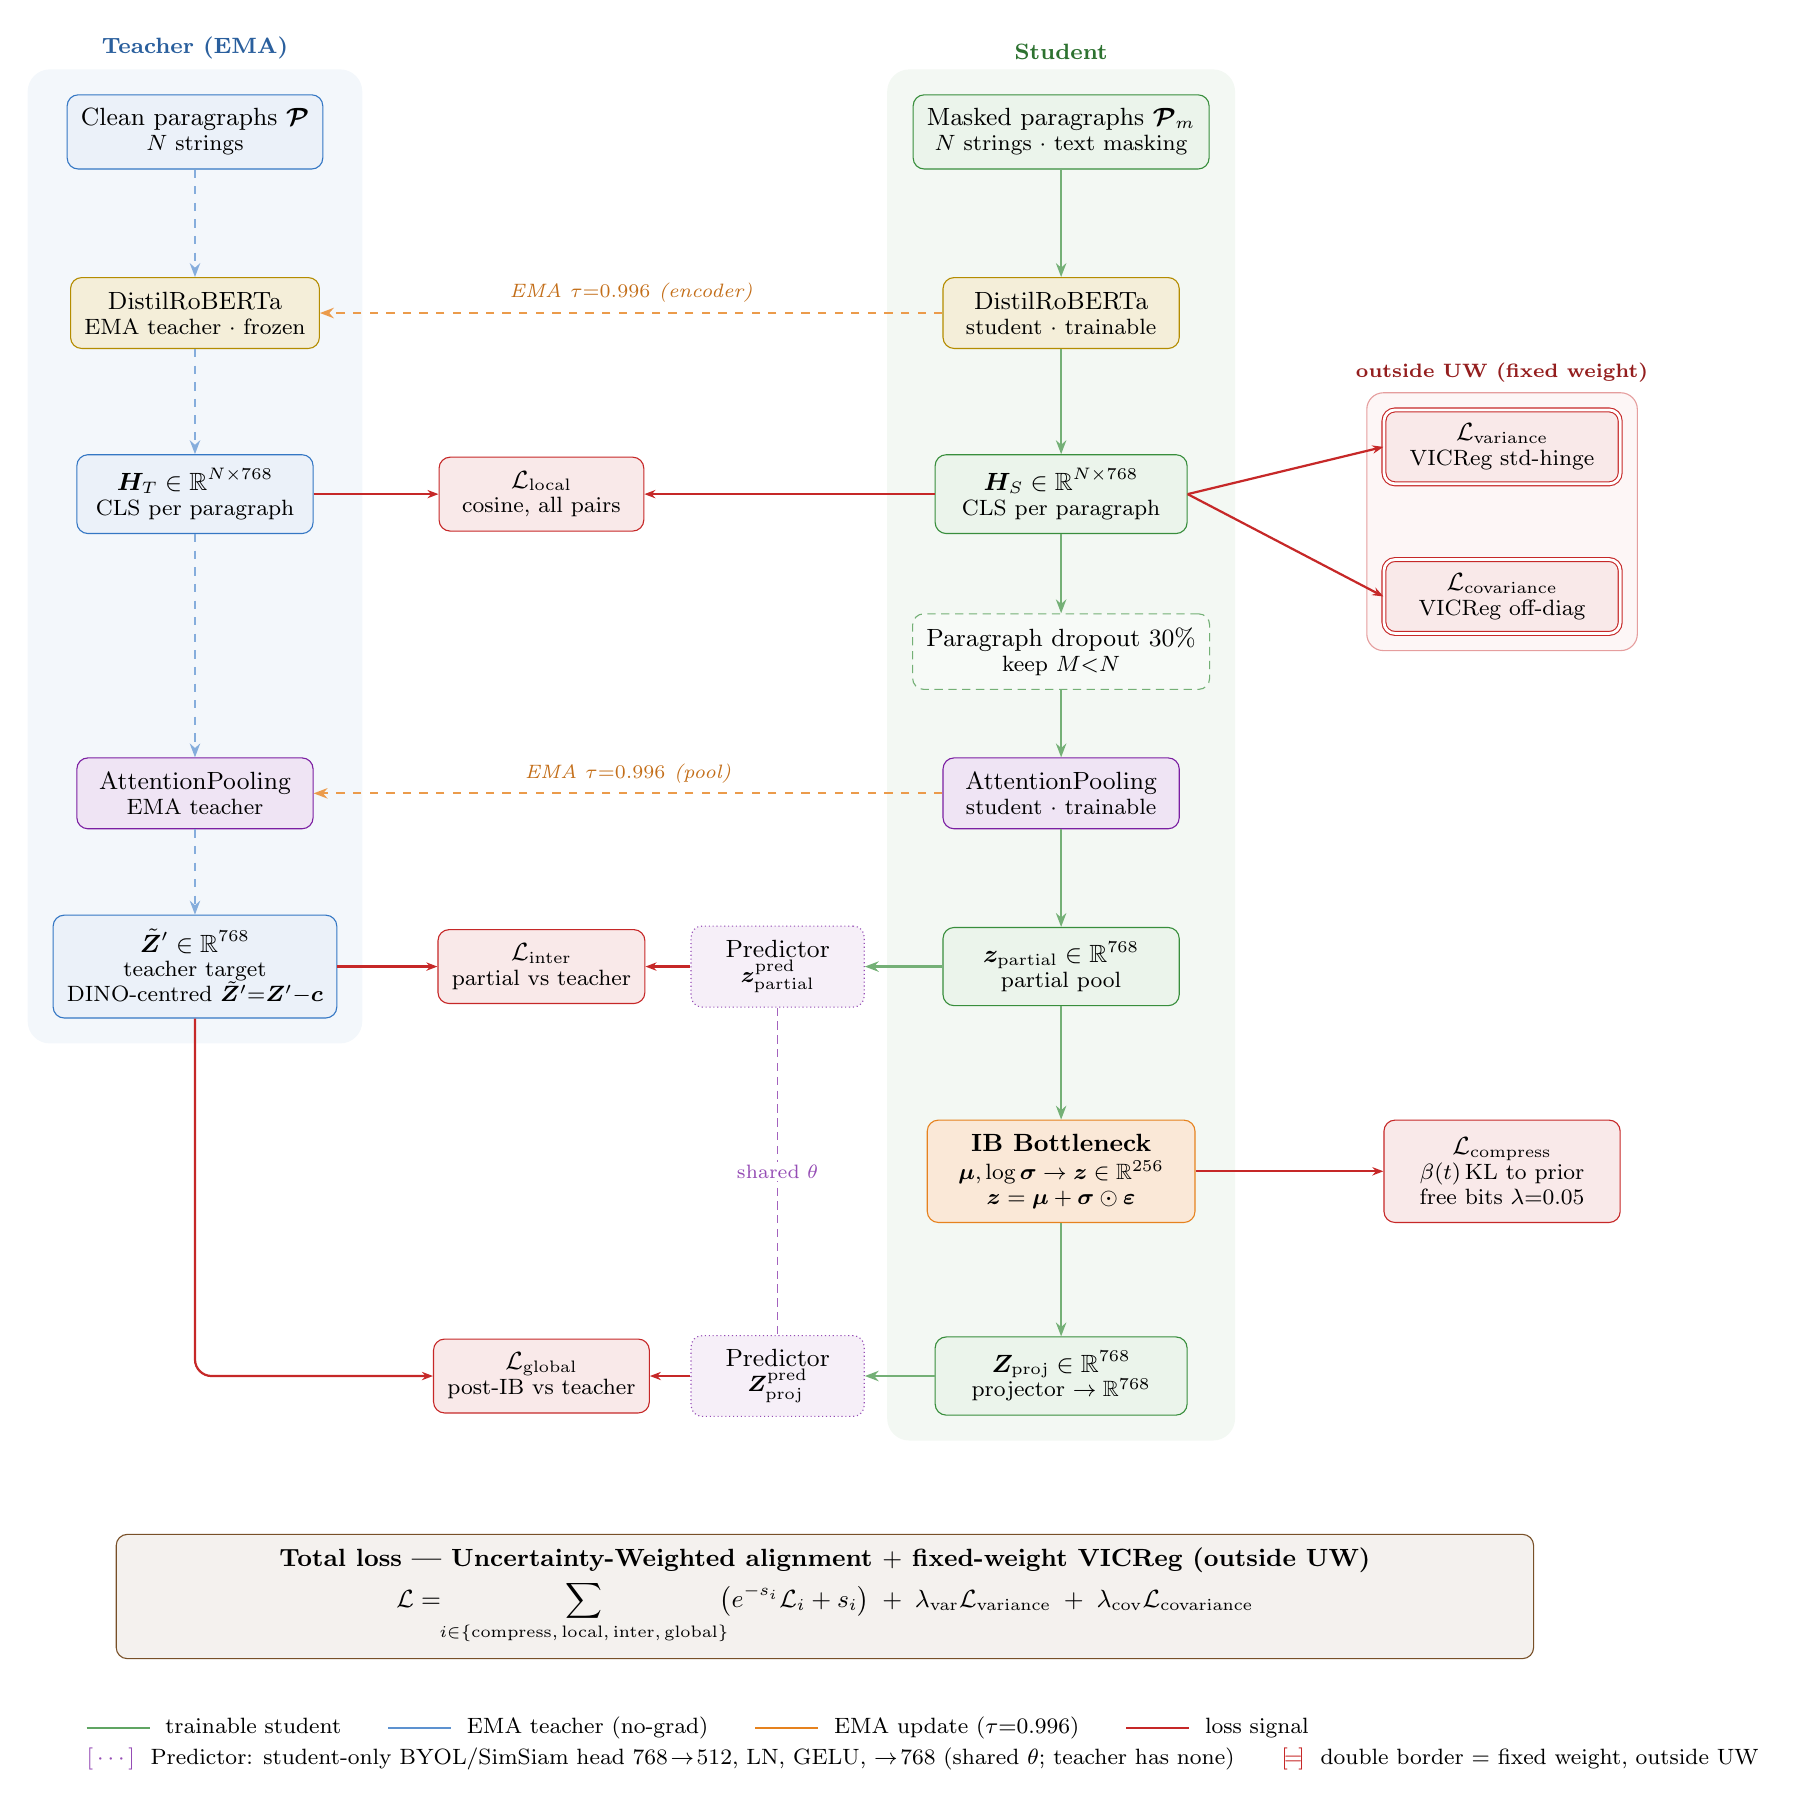
\begin{tikzpicture}

%% ══════════════ TEACHER lane (x = 0) — separate frozen EMA encoder ══════════════
\node[T]   (t_in)  at (0,   0   ) {Clean paragraphs $\bm{\mathcal{P}}$\\[-2pt]\footnotesize $N$ strings};
\node[ENC] (t_enc) at (0,  -2.3 ) {DistilRoBERTa\\[-2pt]\footnotesize EMA teacher $\cdot$ frozen};
\node[T]   (t_cls) at (0,  -4.6 ) {$\bm{H}_T\in\mathbb{R}^{N\times768}$\\[-2pt]\footnotesize CLS per paragraph};
\node[PL]  (t_pl)  at (0,  -8.4 ) {AttentionPooling\\[-2pt]\footnotesize EMA teacher};
\node[T]   (t_zt)  at (0, -10.6 ) {$\tilde{\bm{Z}}'\in\mathbb{R}^{768}$\\[-2pt]\footnotesize teacher target\\[-2pt]\footnotesize DINO-centred $\tilde{\bm{Z}}'{=}\bm{Z}'{-}\bm{c}$};

\draw[Tarr] (t_in)  -- (t_enc);
\draw[Tarr] (t_enc) -- (t_cls);
\draw[Tarr] (t_cls) -- (t_pl);
\draw[Tarr] (t_pl)  -- (t_zt);

%% ══════════════ STUDENT lane (x = 11) — trainable ══════════════
\node[S, minimum width=3.4cm]
           (s_in)  at (11.0,   0   ) {Masked paragraphs $\bm{\mathcal{P}}_m$\\[-2pt]\footnotesize $N$ strings $\cdot$ text masking};
\node[ENC] (s_enc) at (11.0,  -2.3 ) {DistilRoBERTa\\[-2pt]\footnotesize student $\cdot$ trainable};
\node[S, minimum width=3.2cm]
           (s_cls) at (11.0,  -4.6 ) {$\bm{H}_S\in\mathbb{R}^{N\times768}$\\[-2pt]\footnotesize CLS per paragraph};
\node[DR]  (s_dr)  at (11.0,  -6.6 ) {Paragraph dropout $30\%$\\[-2pt]\footnotesize keep $M{<}N$};
\node[PL]  (s_pl)  at (11.0,  -8.4 ) {AttentionPooling\\[-2pt]\footnotesize student $\cdot$ trainable};
\node[S]   (s_zp)  at (11.0, -10.6 ) {$\bm{z}_{\mathrm{partial}}\in\mathbb{R}^{768}$\\[-2pt]\footnotesize partial pool};
\node[IB, minimum width=3.4cm, minimum height=1.3cm]
           (s_ib)  at (11.0, -13.2 ) {\textbf{IB Bottleneck}\\[-1pt]\footnotesize $\bm{\mu},\log\bm{\sigma}\to\bm{z}\in\mathbb{R}^{256}$\\[-2pt]\footnotesize $\bm{z}=\bm{\mu}+\bm{\sigma}\odot\bm{\varepsilon}$};
\node[S, minimum width=3.2cm]
           (s_zj)  at (11.0, -15.8 ) {$\bm{Z}_{\mathrm{proj}}\in\mathbb{R}^{768}$\\[-2pt]\footnotesize projector $\to\mathbb{R}^{768}$};

\draw[Sarr] (s_in)  -- (s_enc);
\draw[Sarr] (s_enc) -- (s_cls);
\draw[Sarr] (s_cls) -- (s_dr);
\draw[Sarr] (s_dr)  -- (s_pl);
\draw[Sarr] (s_pl)  -- (s_zp);
\draw[Sarr] (s_zp)  -- (s_ib);
\draw[Sarr] (s_ib)  -- (s_zj);

%% ══════════════ Student-only PREDICTOR (x = 7.4, shared weights) ══════════════
\node[PRED] (p_a) at (7.4, -10.6) {Predictor\\[-2pt]\footnotesize $\bm{z}_{\mathrm{partial}}^{\mathrm{pred}}$};
\node[PRED] (p_b) at (7.4, -15.8) {Predictor\\[-2pt]\footnotesize $\bm{Z}_{\mathrm{proj}}^{\mathrm{pred}}$};
\draw[Sarr] (s_zp.west) -- (p_a.east);
\draw[Sarr] (s_zj.west) -- (p_b.east);
\draw[densely dashed, pPurple!70] (p_a.south) -- (p_b.north)
      node[midway, fill=white, inner sep=1pt, font=\scriptsize, text=pPurple!80]{shared $\theta$};

%% ══════════════ LOSS SPINE (x = 4.4) — each loss between its operands ══════════════
\node[LO, minimum width=2.6cm] (l_loc) at (4.4,  -4.6) {$\mathcal{L}_{\mathrm{local}}$\\[-2pt]\footnotesize cosine, all pairs};
\draw[Larr] (t_cls.east) -- (l_loc.west);
\draw[Larr] (s_cls.west) -- (l_loc.east);

\node[LO, minimum width=2.6cm] (l_int) at (4.4, -10.6) {$\mathcal{L}_{\mathrm{inter}}$\\[-2pt]\footnotesize partial vs teacher};
\draw[Larr] (t_zt.east) -- (l_int.west);
\draw[Larr] (p_a.west)  -- (l_int.east);

\node[LO, minimum width=2.6cm] (l_glb) at (4.4, -15.8) {$\mathcal{L}_{\mathrm{global}}$\\[-2pt]\footnotesize post-IB vs teacher};
\draw[Larr] (p_b.west) -- (l_glb.east);
\draw[Larr, rounded corners=6pt] (t_zt.south) |- (l_glb.west);   %% single teacher-target rail

%% ══════════════ REGULARIZERS (x = 16.6) — clearly separated right lane ══════════════
\node[LO, minimum width=3.0cm, minimum height=1.3cm]
      (l_cmp) at (16.6, -13.2) {$\mathcal{L}_{\mathrm{compress}}$\\[-2pt]\footnotesize $\beta(t)\,\mathrm{KL}$ to prior\\[-2pt]\footnotesize free bits $\lambda{=}0.05$};
\draw[Larr] (s_ib.east) -- (l_cmp.west);

\node[LOX] (l_var) at (16.6,  -4.0) {$\mathcal{L}_{\mathrm{variance}}$\\[-2pt]\footnotesize VICReg std-hinge};
\node[LOX] (l_cov) at (16.6,  -5.9) {$\mathcal{L}_{\mathrm{covariance}}$\\[-2pt]\footnotesize VICReg off-diag};
\draw[Larr] (s_cls.east) -- (l_var.west);
\draw[Larr] (s_cls.east) -- (l_cov.west);

%% ══════════════ EMA links (student -> teacher): encoder AND pool ══════════════
\draw[EMA] (s_enc.west) -- (t_enc.east)
      node[midway, above, font=\scriptsize\itshape, text=ibOrange!85!black]{EMA $\tau{=}0.996$ (encoder)};
\draw[EMA] (s_pl.west) -- (t_pl.east)
      node[midway, above, font=\scriptsize\itshape, text=ibOrange!85!black]{EMA $\tau{=}0.996$ (pool)};

%% ══════════════ TOTAL LOSS (compact banner) ══════════════
\node[TOT, minimum width=18cm, minimum height=1.2cm, align=center]
      (l_tot) at (8.0, -18.6) {%
      \textbf{Total loss --- Uncertainty-Weighted alignment $+$ fixed-weight VICReg (outside UW)}\\[2pt]
      $\displaystyle \mathcal{L}=\!\!\sum_{i\in\{\mathrm{compress},\,\mathrm{local},\,\mathrm{inter},\,\mathrm{global}\}}\!\!\bigl(e^{-s_i}\mathcal{L}_i+s_i\bigr)\;+\;\lambda_{\mathrm{var}}\mathcal{L}_{\mathrm{variance}}\;+\;\lambda_{\mathrm{cov}}\mathcal{L}_{\mathrm{covariance}}$};

%% ══════════════ BACKGROUND PANELS (fit, auto-sized) ══════════════
\begin{scope}[on background layer]
  \node[fill=tBlue!6, rounded corners=8pt, fit=(t_in)(t_enc)(t_cls)(t_pl)(t_zt), inner sep=9pt] (tpanel){};
  \node[fill=sGreen!6, rounded corners=8pt, fit=(s_in)(s_enc)(s_cls)(s_dr)(s_pl)(s_zp)(s_ib)(s_zj), inner sep=9pt] (spanel){};
  \node[draw=lossRed!45, fill=lossRed!4, rounded corners=6pt, fit=(l_var)(l_cov), inner sep=6pt] (uwbox){};
\end{scope}
\node[font=\bfseries\footnotesize, text=tBlue!80!black, anchor=south] at (tpanel.north) {Teacher (EMA)};
\node[font=\bfseries\footnotesize, text=sGreen!80!black, anchor=south] at (spanel.north) {Student};
\node[font=\bfseries\scriptsize, text=lossRed!75!black, anchor=south] at (uwbox.north) {outside UW (fixed weight)};

%% ══════════════ LEGEND ══════════════
\node[font=\footnotesize, anchor=north west, align=left] at (-1.5,-20.0) {%
  \textcolor{sGreen!80}{\rule[0.4ex]{0.8cm}{0.7pt}}~ trainable student\qquad
  \textcolor{tBlue!80}{\rule[0.4ex]{0.8cm}{0.7pt}}~ EMA teacher (no-grad)\qquad
  \textcolor{ibOrange}{\rule[0.4ex]{0.8cm}{0.7pt}}~ EMA update ($\tau{=}0.996$)\qquad
  \textcolor{lossRed}{\rule[0.4ex]{0.8cm}{0.7pt}}~ loss signal\\[2pt]
  \textcolor{pPurple!80}{$[\,\cdots\,]$}~ Predictor: student-only BYOL/SimSiam head $768\!\to\!512$, LN, GELU, $\to\!768$ (shared $\theta$; teacher has none)\qquad
  \textcolor{lossRed}{$[\!=\!]$}~ double border $=$ fixed weight, outside UW};

\end{tikzpicture}
\end{document}
